\documentclass[10pt,conference]{IEEEtran}

\usepackage[T1]{fontenc}
\usepackage[utf8]{inputenc}
\usepackage[table]{xcolor}
\usepackage{graphicx}
\usepackage{float}

\usepackage{booktabs}
\usepackage{multirow}
\usepackage{parcolumns}

\usepackage{todonotes}
\usepackage{amsmath}
\usepackage{amssymb}


\def\checkmark{\tikz\fill[scale=0.4](0,.35) -- (.25,0) -- (1,.7) -- (.25,.15) -- cycle;}

\definecolor{pblue}{rgb}{0.13,0.13,1}
\definecolor{pgreen}{rgb}{0,0.5,0}
\definecolor{pred}{rgb}{0.9,0,0}
\definecolor{pgrey}{rgb}{0.46,0.45,0.48}

\usepackage{listings}
\lstset{language=Java,
  showspaces=false,
  showtabs=false,
  breaklines=true,
  showstringspaces=false,
  breakatwhitespace=true,
  commentstyle=\color{pgreen},
  keywordstyle=\color{pblue},
  numbers = left,
  stringstyle=\color{pred},
  basicstyle=\ttfamily,
  moredelim=[il][\textcolor{pgrey}]{\$\$},
  moredelim=[is][\textcolor{pgrey}]{\%\%}{\%\%}
}

\definecolor{lightyellow}{HTML}{fffdcc}
\definecolor{doublelightyellow}{HTML}{fffa9c}
\definecolor{lightgreen}{HTML}{dcffd4}
\definecolor{lightblue}{HTML}{e0ffff}
\definecolor{lightred}{HTML}{ffe0e0}
\definecolor{lightpink}{HTML}{ffe0ff}
\definecolor{lightorange}{HTML}{ffede0}
\definecolor{lightpurple}{HTML}{f0e0ff}
\newcommand{\highlightYellow}{\makebox[0pt][l]{\color{lightyellow}\rule[-4pt]{1\linewidth}{14pt}}}
\newcommand{\highlightGreen}{\makebox[0pt][l]{\color{lightgreen}\rule[-4pt]{1\linewidth}{14pt}}}
\newcommand{\highlightBlue}{\makebox[0pt][l]{\color{lightblue}\rule[-4pt]{1\linewidth}{14pt}}}
\newcommand{\highlightRed}{\makebox[0pt][l]{\color{lightred}\rule[-4pt]{1\linewidth}{14pt}}}
\newcommand{\highlightPink}{\makebox[0pt][l]{\color{lightpink}\rule[-4pt]{1\linewidth}{14pt}}}
\newcommand{\highlightOrange}{\makebox[0pt][l]{\color{lightorange}\rule[-4pt]{1\linewidth}{14pt}}}
\newcommand{\highlightPurple}{\makebox[0pt][l]{\color{lightpurple}\rule[-4pt]{1\linewidth}{14pt}}}
\newcommand{\highlightDarkyellow}{\makebox[0pt][l]{\color{doublelightyellow}\rule[-4pt]{1\linewidth}{14pt}}}

\lstnewenvironment{javacode}[1][]{\lstset{language=Java,escapechar=|,tabsize=2, breaklines=true, xleftmargin=.25in, keywordstyle=\color{pblue},basicstyle=\small,#1}}{}

\begin{document}

\title{Improving Software Maintainability through automatic refactoring of Code Clones}
\author{}
\maketitle
\thispagestyle{plain} % This is for page numbers, remove before submit
\pagestyle{plain}


%\author{Simon Baars}
%\affiliation{\institution{University of Amsterdam}}
%\email{simon.mailadres@gmail.com}

%\author{Ana Oprescu}
%\affiliation{\institution{University of Amsterdam}}
%\email{a.m.oprescu@uva.nl}

\begin{abstract}
Duplication in source code is often seen as one of the most harmful types of technical debt as it increases the size of the codebase and creates implicit dependencies between fragments of code. To remove such anti-patterns, the codebase should be refactored. Many tools aid in the de©tection process of such duplication problems but do not determine whether refactoring an identified clone would improve the maintainability.

We address this shortcoming by first analyzing what preconditions apply to be able to refactor clones. We then propose a tool to detect clones, analyze their context and automatically refactor a subset of them. We use a set of established metrics to determine the impact of the applied refactorings on the maintainability of the system. Based on these results, one could decide which clones would improve system design if refactored. We evaluate our approach over a large corpus of open-source Java projects.

We identify the factors of interest characterizing the impact on maintainability of automatically applied refactorings. We find that the biggest influencing factor is token volume. We define token volume as the combined number of tokens in all clone instances in a clone class. The majority of duplicates with a token volume of 63 or more tokens improve maintainability when refactored. The amount of external data that needs to be passed to the merged location of the duplicate is the other important factor: the majority of clones requiring more than two external parameters decrease maintainability.
\end{abstract}

\begin{IEEEkeywords}
code clones, refactoring, static code analysis, object-oriented programming
\end{IEEEkeywords}

\maketitle

\section{Introduction}
Duplicate fragments in source code (also named ``code clones'') are often seen as one of the most harmful types of technical debt~\cite{fowler2018refactoring}. Duplicate fragments create implicit dependencies that make the code harder to maintain as the resolution of erroneous behavior in one location may have to be applied to all the cloned code as well~\cite{ostberg2014automatically}. Apart from that, code clones can contribute up to 25\% of the code size~\cite{bruntink2005use}.

%Clone detection tools often use thresholds to determine which clones should be considered. Most clone detection tools use the number of lines \cite{kamiya2002ccfinder, svajlenko2016bigcloneeval}, statements \cite{higo2013revisiting, kamalpriya2017enhancing} and/or tokens \cite{ragkhitwetsagul2019siamese, jiang2007deckard} as thresholds to determine whether clones should be considered. We outline the shortcomings of these thresholds to find clones such that the maintainability of the source code is improved when refactored, and propose new thresholds to control this characteristic.
% Current clone detection techniques are limited to measuring the size of clones to determine whether they should be considered. Because of this, the output of clone detection tools is often of limited assistance to the developer in the refactoring process.
To reduce duplication of a codebase, there are several refactoring techniques that can be applied. The most used refactoring technique to deal with code clones is ``Extract Method'' \cite{fowler2018refactoring}. This technique entails that the duplicated code is moved to a new method, which is then called from all locations where the duplicated code was used. To be able to execute such a refactoring, several preconditions apply \cite{tsantalis2015assessing}.
\todo[inline]{still missing link on how current solutions do not help improving maintainability - our message from monday night is not crystal clear yet}
In this study, we analyze which preconditions apply to determine whether a clone could and should be automatically refactored. We list criteria that influence the maintainability of clones when refactored. We evaluate the context of clones to determine which refactoring techniques are best suited. We define the context of clones as the inheritance relation between clone instances in a clone class and the location of clone instances in the codebase. We showcase the proposed technique as a tool that automatically refactors clones by extracting new methods out of duplicated code.

We measure several maintainability metrics before and after refactoring to determine the impact on system maintainability of applying the refactoring. These metrics are volume, method parameters, duplication and complexity. Using this setup, we gain empirical data about the maintainability improvement of clones on a large set of data in a controlled environment. Because the refactoring is done automatically, we also consider micro-clones, which are shown to be important for refactoring consideration \cite{mondai2018micro}. We use this data to define which characteristics of clones have the biggest influence of system maintainability when such a clone is refactored. This allows for more a accurate suggestion of code clones for refactoring and can assist in the refactoring process.

Most clone detection tools can be configured using thresholds. These thresholds indicate the minimum number of lines, tokens and/or statements that must be spanned for duplicate fragments to be considered clones. Often, such thresholds are intuitively chosen~\cite{li2006cp, roy2009mutation} or based on a quartile distribution of empirical data~\cite{alves2010deriving}. Using the maintainability score we can find support for which thresholds should be chosen to increase the chance to find clones that improve maintainability when refactored. %TODO: Check whether this really fits here

Over a corpus of 2.267 Java project our tool refactored 12.710 clone classes. We found that the main influencing factor on maintainability when refactored is token volume. We define token volume as the combined number of tokens in all clone instances in a clone class. When refactoring clones with a very small token volume, we found that the maintainability decreases when such clones are refactored. The average clone with a clone volume of 65 or larger improves maintainability when refactored. The other factor with a major influence on maintainability is the number of parameters that are required for the extracted method. We found that if a clone requires more than 2 parameters in the extracted method, it is more likely to decrease maintainability.

This paper is organized as follows. In Sec.~\ref{sec:background} we revisit key clone refactoring background. Sec.~\ref{sec:relatedwork} discusses state-of-the-art in automated clone refactoring research. In Sec.~\ref{sec:research} we propose a definition for clones such that they could and should be automatically refactored. In Sec.~\ref{sec:clonerefactor} we introduce our clone refactoring tool. In Sec.~\ref{sec:experimentalsetup} we explain the setup of our experiments; we show the results in Sec.~\ref{sec:results} and discuss them in Sec.~\ref{sec:discussion}.
%We evaluate our approach by comparing the maintainability of before- and after snapshots of a codebase for each duplication problem that is refactored. We define which factors have the greatest influence on whether a clone improves maintainability when refactored. We find a set of thresholds by which clones can be detected that are more likely to improve maintainability when refactored. This allows for more a accurate suggestion of code clones for refactoring and can assist in the refactoring process.

\section{Background}\label{sec:background}
We briefly describe relevant code clone and clone refactoring research.

\subsection{Code clones}
We use two concepts to argue about code clones~\cite{roy2007survey}:
\\ \textbf{Clone instance}: A single cloned fragment.
\\ \textbf{Clone class}: A set of similar clone instances.

%\subsection{Clone Types}
Duplication in code is found in many different forms. Most often duplicated code is the result of a programmer reusing previously written code \cite{haefliger2008code, baxter1998clone}. Sometimes this code is then adapted to fit the new context. To reason about these modifications, several clone types have been proposed%. These clone types are described in Roy et al
~\cite{roy2007survey}:\\
\textbf{Type I:} Identical code fragments except for variations in whitespace (may be also variations in layout), and comments.\\
\textbf{Type II:} Structurally/syntactically identical fragments except variations in identifiers, literals, types, layout, and comments.\\
\textbf{Type III:} Copied fragments with further modifications. Statements can be changed, added or removed next to variations in identifiers, literals, types, layout, and comments.
A higher type of clone means that it is harder to detect and refactor. Many studies adopt these clone types, analyzing them further and writing detection techniques for them \cite{sajnani2016sourcerercc, kodhai2010detection, van2019novel}.

\subsection{Clone Refactoring}
\subsubsection{Refactoring techniques}
The most common technique for refactoring clones is ``Extract Method''~\cite{fowler2018refactoring}, which can be applied on code inside the body of a method. Applying this technique entails moving functionality from the body of a method to a new method. To reduce duplication with this technique, the contents of a single clone instance are extracted to a new method and all further locations of the clone are replaced by a call to the new method.

\subsubsection{Preconditions}
Clones detected by current detection techniques \cite{kamiya2002ccfinder, deissenboeck2010flexible, jiang2007deckard, cordy2011nicad} are subject to a set of preconditions to determine whether they can be refactored \cite{tsantalis2015assessing}:
\begin{enumerate}
  \item The parameterization of differences between the matched statements should not break existing data-, anti-, and output-dependencies.
  \item The unmatched statements should be movable before or after the matched statements without breaking existing data-, anti-, and output-dependencies.
  \item The duplicated code fragments should return at most one variable of the same type.
  \item Matched branching (\texttt{break}, \texttt{continue}) statements should be accompanied with corresponding matched loop statements.
  \item Matched variables having different subclass types should call only methods that are declared in the common superclass or are being overridden in the respective subclasses.
  \item The parameterization of fields belonging to differences between the mapped statements is possible only if they are not modified.
  \item The parameterization of method calls belonging to differences between the mapped statements is possible only if they do not return a void type.
  \item The mapped statements within the clone fragments should not contain any conditional return statements.
\end{enumerate}

\begin{figure*}
\begin{parcolumns}{2}
\colchunk[1]{
\begin{javacode}
package com.sb.game;

import java.util.List;

public class GameScene
{
|\highlightYellow|	public void addToList(List l) {
|\highlightYellow|		l.add(getClass().getName());
|\highlightYellow|	}

	public void addTen(int x) {
|\highlightYellow|		x = x + 10; // Addition
|\highlightYellow|		Notifier.notifyChanged(x);
|\highlightYellow|		return x;
	}
}
\end{javacode}}
\colchunk[2]{
\begin{javacode}
package com.sb.fruitgame;

import java.awt.List; // Different type

public class LoseScene
{
|\highlightYellow|	public void addToList(List l) {
|\highlightYellow|		l.add(getClass().getName());
|\highlightYellow|	}

	public void concatTen(String x) {
|\highlightYellow|		x = x + 10; // String concatenation
|\highlightYellow|		Notifier.notifyChanged(x);
|\highlightYellow|		return x;
	}
}
\end{javacode}}
\end{parcolumns}
\caption{Example of textually equal code fragments that differ in functionality.}
\label{fig:type1}
\end{figure*}

\section{Related Work}\label{sec:relatedwork}
We outline relevant research to clone refactoring. A significant aspect is the context of clones.

\subsection{Clone context analysis}\label{sec:rw:contextanalysis}
Golomingi~\cite{koni2001scenario} explores mapping the relation between clone instances to refactoring methods. The author analyses the refactoring methods described by Martin Fowler \cite{fowler1999refactoring} and analyzes what refactoring methods can be used to refactor clones with what inheritance relations. The identified clone relations are: Ancestor, Common Hierarchy, First Cousin, Same Method, Sibling, Single Class, Superclass and Unrelated. We extend this list with several more fine-grained relations, suitable for automatic refactoring (see Sec.~\ref{sec:relation}).

Fontana et al.~\cite{fontana2012duplicated, fontana2015duplicated} combine the research by Golomingi~\cite{koni2001scenario} with clone types 1 and 3 \cite{roy2007survey}. They use a large corpus~\cite{tempero2010qualitas} on which they perform statistical analyses of clone relations together with clone types. We repeat this research with a vastly different setup: we use the clone definition from Sec.~\ref{sec:research} and the relation categories outlined in Sec.~\ref{sec:relation}.

\subsection{Clone refactoring}
Krishnan et al.~\cite{krishnan2013refactoring} approach clone refactoring as an optimization problem: how variability between cloned fragments influences the refactoring techniques required and their implications on system design. The main focus of this study is to find out which clones \textbf{can} be refactored. We extend this work by looking into which clones \textbf{should} be refactored. We propose definitions for refactorable clones together with thresholds to be able to limit their negative impact on system design. We measure which clones improve maintainability when refactored. This results in a set of thresholds that can be used to detect and refactor clones that should be refactored.
%The state-of-the-art in code clone refactoring is the work by Mazinanian et al.~\cite{mazinanian2016jdeodorant}. The authors propose a tool named JDeodorant that can automatically refactor a subset of duplication problems. This tool is based on several studies that look into different aspects of code clone refactoring. In a study by Krishnan et al.~\cite{krishnan2013refactoring} clone refactoring is approached as an optimization problem: how variability between cloned fragments influences the refactoring techniques required and their implications on system design. Another study by Krishnan et al.~\cite{krishnan2014unification} proposes a list of preconditions for clones to determine their refactorability. This list is revised by Tsantalis et al.~\cite{tsantalis2015assessing}, proposing a set of 8 preconditions that determine whether two duplicated fragments can be refactored.

%A recent study~\cite{tsantalis2017clone} looks into how lambdas can assist the clone refactoring process.

\section{Defining refactorable clones}\label{sec:research}
%In literature, several clone type definitions have been used to argue about duplication in source code~\cite{roy2007survey}.
We discuss how we can define clones such that they can be automatically refactored while avoiding changing the functional behavior and other negative side effects on the source code, such as decreasing the maintainability of the code.

\subsection{Ensuring equality}\label{sec:t1r}
Most modern clone detection tools detect duplication by comparing the code textually together with the omission of certain tokens~\cite{roy2009comparison, svajlenko2014evaluating}. Clones detected by such means may not always be suitable for refactoring, because textual comparison fails to take into account the context of certain symbols in the code. Information that gets lost in textual comparison is the referenced declaration for type, variable and method references. Equally named type, variable and method references may refer to different declarations with a different implementation (Fig~\ref{fig:type1} shows an example of this). Such clones can be harder to refactor, if beneficial at all.

To detect automatically refactorable clones, we propose to:
\begin{itemize}
  \item Compare types by their fully qualified identifier (FQI). The FQI of a type reference describes the full path to where it is declared.
  \item Compare variable references not only by their name but also by their type (FQI).
  \item Compare method references by their fully qualified signature (FQS). The FQS of a method reference describes the full path to where it is declared, plus the FQI of the type of each of its parameters.
\end{itemize}

\subsection{Allowing variability in a controlled set of expressions} \label{sec:t2r}
Often, duplication fragments in source code do not match exactly~\cite{kodhai2013method}. When developers duplicate fragments of code, they modify the duplicated block to fit its new location and purpose. To detect duplicate fragments with minor variance, we look into what expressions we can allow variability in, while still being automatically refactorable.

We define the following expressions as automatically refactorable when varied:
\begin{itemize}
  \item \textbf{Literals}: Only if all varying literals in a clone class have the same type.
  \item \textbf{Variables}: Only if all varying variables in a clone class have the same type.
  \item \textbf{Method references}: Only if the return value of referenced methods match (or are not used).
\end{itemize}
Often when allowing such variance, trade-offs come into play~\cite{krishnan2013refactoring, krishnan2014unification}. For instance, variance in literals may require the introduction of a parameter to an extracted method if the ``Extract Method'' refactoring method is used, increasing the required effort to comprehend the code \cite{heitlager2007practical}.

\subsection{Gapped clones} \label{sec:t3r}
Sometimes, when fragments are duplicated, a statement is inserted or changed severely for the code to fit its new context~\cite{roy2007survey}. When dealing with such situations, there are several opportunities to refactor so-called ``gapped clones''~\cite{ueda2002detection, zhao2018automatic}. ``Gapped clones'' are two clone instances separated by a ``gap'' of non-cloned statement(s). We define the following methods to refactor such clones, based on research by Tsantalis et al~\cite{tsantalis2015assessing}:
\begin{itemize}
  \item Wrap the difference in statements in a conditionally executed block, one path for each different (group of) statement(s).
  \item Use a lambda function to pass the difference in statements from each location of the clone~\cite{tsantalis2017clone}.
\end{itemize}
For both of these techniques, a trade-off is at play. This is because these solutions increase the complexity and volume of the source code in favor of removing a clone.

\section{Survey existing clone detection tools}\label{sec:survey}
%To detect refactorable clones according to the definitions introduced in Sec.~\ref{sec:research}, we survey existing clone detection tools for their suitability.
To investigate the impact of the definitions introduced in Sec.~\ref{sec:research}, we need a tool to detect refactorable clones according to these definitions. We conducted a short survey on (recent) clone detection tools to detect such clones that can be refactored. The results of our survey are displayed in table~\ref{table:dettools}. We chose a set of tools that are open source and can analyze a popular object-oriented programming language. Next, we formulate the following four criteria by which we analyze these tools:
\begin{enumerate}
    \item \textbf{Should find clones in any context.} Some tools only find clones in specific contexts, such as only method level clones. We want to perform an analysis of all clones in projects to get a complete overview.
\item \textbf{Finds clone classes in control projects.} We assembled a number of control projects to assess the validity of the surveyed clone detection tools.
\item \textbf{Can analyze resolved symbols.} When detecting the types proposed in Sec.~\ref{sec:rtypes}, it is important that we can analyze resolved symbols (for instance a type reference). The rationale for this is further explained in~\ref{chap:challenge}.
\item \textbf{Extensive detection configuration.} Detecting our clone definitions, as proposed in Sec.~\ref{sec:rtypes}, require to have some understanding about the meaning of tokens in the source code (whether a certain token is a type, variable, etc.). The tool should recognize such structures, in order for us to configure our clone type definitions in the tool.
\end{enumerate}

\begin{table}[H]
 \begin{center}
  \caption{Our survey on clone detection tools.} \label{table:dettools}
  \medskip
\begin{tabular}{|l|l|l|l|l|l|}
\hline
\textbf{Clone Detection Tool} & \textbf{(1)} & \textbf{(2)} & \textbf{(3)} & \textbf{(4)} \\ \hline
Siamese~\cite{ragkhitwetsagul2019siamese} &  &             &             & \checkmark            \\ \hline
NiCAD~\cite{roy2008nicad, cordy2011nicad} & \checkmark                             & \checkmark            &             &             \\ \hline
CPD~\cite{roy2009comparison} & \checkmark & \checkmark            &             &             \\ \hline
\begin{tabular}[c]{@{}l@{}}CCFinder~\cite{kamiya2002ccfinder}\\ D-CCFinder~\cite{livieri2007very}\end{tabular} & \checkmark  & \checkmark   &    &   \\ \hline
CCFinderSW~\cite{semura2017ccfindersw}   & \checkmark     &             &             & \checkmark            \\ \hline
\begin{tabular}[c]{@{}l@{}}SourcererCC~\cite{sajnani2016sourcerercc}\\ Oreo~\cite{saini2018oreo}\end{tabular} & \checkmark    &             &             & \checkmark            \\ \hline
BigCloneEval~\cite{svajlenko2016bigcloneeval}  & \checkmark  & \checkmark   &             &             \\ \hline
Deckard~\cite{jiang2007deckard} & \checkmark   &             & \checkmark            &             \\ \hline
Scorpio~\cite{higo2013revisiting, kamalpriya2017enhancing} & \checkmark   &     & \checkmark  & \checkmark   \\ \hline
\end{tabular}
\end{center}
\end{table}

Apart from these criteria, we found that the output of these clone detection tools cannot be post-processed to find the clone definition proposed in Sec.~\ref{sec:research}. This is mainly because these clones are not necessarily a subset of clones detected by these tools and will thus require an analysis of the entire system.

%To detect clones that can be automatically refactored, we surveyed a set of modern clone detection tools and techniques~\cite{svajlenko2014evaluating, sheneamer2016survey, gautam2016various, roy2009comparison}. We created a set of control projects to determine the suitability of these tools to detect automatically refactorable clones, either through configuration or postprocessing of their output.

%None of the surveyed tools~\cite{ragkhitwetsagul2019siamese, roy2008nicad, semura2017ccfindersw, sajnani2016sourcerercc, saini2018oreo, jiang2007deckard, kamalpriya2017enhancing, mazinanian2016jdeodorant} were suitable for our definitions of refactorable clones, because of which we propose CR. This tool goes through a 3-step process to automatically refactor clones as shown in Fig.~\ref{fig:clonerefactorflow}. In the following sections, we explain these steps.

\section{A tool for automatic clone refactoring}\label{sec:clonerefactor}
None of the surveyed tools were suitable for our definitions of refactorable clones. Therefore, we built a new tool, CR\footnote{Name anonymized for the blind review, camera-ready paper would include a link to the GitHub repo of the tool.} This tool goes through a 3-step process to automatically refactor clones as shown in Fig.~\ref{fig:clonerefactorflow}. In Sec.~\ref{sec:detection} we describe how CR detects refactorable clones. In Sec.~\ref{sec:context} we describe how CR maps the context of clones as input for the refactoring process described in Sec.~\ref{sec:refactoring}.

\begin{figure}[H]
  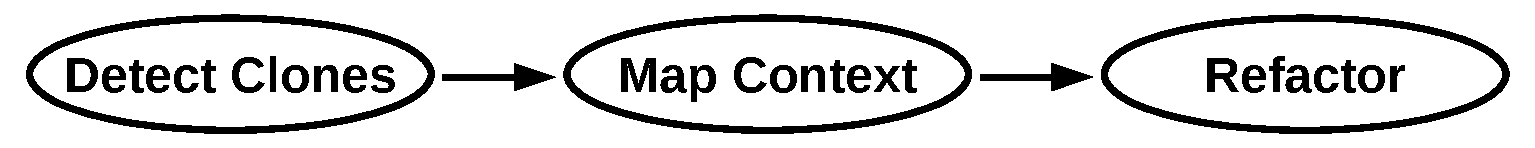
\includegraphics[width=1\columnwidth]{img/flow}
  \caption{Abstract flow diagram of CR.}
  \label{fig:clonerefactorflow}
\end{figure}

\subsection{Clone detection}\label{sec:detection}
We use an AST-based method to detect clones. Clones are detected on a statement level: only full statements are considered as clones. In Sec.~\ref{sec:t2r} we described that we limit the variability between variable, literal and method reference expressions by a threshold. This threshold is the percentage of different expressions against the total number of expressions in the source code:
\begin{equation}\label{eq:type2r}
\text{Variability}=\frac{\text{Different expressions}}{\text{Total expressions}}*100
\end{equation}

After all clones have been detected, CR determines whether clone classes can be merged into gapped clones (see Sec.~\ref{sec:t3r}). The maximum size of the gap is limited by a threshold. This threshold is the percentage of (not-cloned) statements in the gap against the sum of statements in both clones surrounding it:
\begin{equation}\label{eq:type3r}
\text{Gap Size}=\frac{\text{Statements in gap}}{\text{Statements in clones}}*100
\end{equation}

Note that unlike the expression variability threshold, this threshold can exceed 100\%. This is because, in theory, the gap can be larger than the clones surrounding it.

% To verify the correctness of all detected clones, we ran the tool over a large project and manually checked the output. We also created a set of control projects to test the correctness for many edge cases.

\begin{figure*}
\begin{parcolumns}{2}
\colchunk[1]{
\begin{javacode}
|\highlightYellow|int a = getA();
|\highlightYellow|while(a<1000) {
|\highlightYellow|  a *= 5;
  doC();
}
\end{javacode}}
\colchunk[2]{
\begin{javacode}
|\highlightYellow|int a = getA();
|\highlightYellow|while(a<1000) {
|\highlightYellow|  a *= 5;
  doB(a);
}
\end{javacode}}
\end{parcolumns}
\caption{A clone that spans a block partially.}
\label{fig:refactorabilitypartialblock}
\end{figure*}

\subsection{Context mapping} \label{sec:context}
After clones are detected, we map the context of these clones. We identify two properties of clones as their context: relation~\cite{fontana2012duplicated} and location~\cite{tairas2011representing}. We identify categories for each of these properties, to get a detailed insight into the context of clones.

\subsubsection{Relation}\label{sec:relation}
Clone instances in a clone class may have a relation with each other through inheritance. This relation has a big impact on how the clone should be refactored~\cite{fontana2015duplicated}. We define the following categories to map the relation between clone instances in a clone class, partly derived from Fontana et al~\cite{fontana2015duplicated} (see Sec~\ref{sec:rw:contextanalysis}). These categories do not map external classes (classes outside the project, e.g. belonging to a library) unless explicitly stated:
\begin{itemize}
    \item \textbf{Common Class}: All clone instances are in the same class.
    \begin{itemize}
        \item \textbf{Same Method}: All clone instances are in the same method.
        \item \textbf{Same Class}: All clone instances are in the same class.
    \end{itemize}
    \item \textbf{Common Hierarchy}: All clone instances are in the same inheritance hierarchy.
    \begin{itemize}
        \item \textbf{Superclass}: Clone instances reside in a class or its parent class.
        \item \textbf{Sibling Class}: All clone instances reside in classes with the same parent class.
        \item \textbf{Ancestor Class}: All clone instances reside in a class, or any of its recursive parents.
        \item \textbf{First Cousin}: All clone instances reside in classes with the same grandparent class.
        \item \textbf{Same Hierarchy}: All clone instances are part of the same inheritance hierarchy.
    \end{itemize}
    \item \textbf{Common Interface}: All clone instances are in classes that have the same interface.
    \begin{itemize}
        \item \textbf{Same Direct Interface}: All clone instances are in classes that have the same interface.
        \item \textbf{Same Class}: All clone instances are in an inheritance hierarchy that contains the same interface.
    \end{itemize}
    \item \textbf{Unrelated}: All clone instances are in classes that have the same interface.
    \begin{itemize}
        \item \textbf{No Direct Superclass}: All clone instances are in classes that have the Object class as their parent.
        \item \textbf{No Indirect Superclass}: All clone instances are in a hierarchy that contains a class that has the Object class as their parent.
        \item \textbf{External Superclass}: All clone instances are in classes the same external class as their parent.
        \item \textbf{Indirect External Ancestor}: All clone instances are in a hierarchy that contains a class that has an external class as their parent.
    \end{itemize}
\end{itemize}

Based on these relations, CR determines where to place the cloned fragment when extracted to a new method. These categories are mutually exclusive: a clone class is flagged as the first relation in the above list that it applies to. The code of clones that have a \textit{Common Class} relation can be refactored by placing the cloned code in this same class~\cite{fowler2018refactoring}. The code of clones with a \textit{Common Hierarchy} relation can be placed in the intersecting class in the hierarchy (the class all clone instances have in common as an ancestor)~\cite{fowler2018refactoring}. The code of clones with a \textit{Common Interface} relation can be placed in the intersecting interface~\cite{mohnen2002interfaces}, but in the process has to become part of the classes' public contract. The code of clones that are \textit{Unrelated} can be placed in a newly created place. The state-of-the-art uses a utility class~\cite{mazinanian2016jdeodorant}, whereas CR creates a new superclass or interface abstraction. The reason CR creates a superclass or interface rather than a utility class is that it makes the relation explicit and allows previously unrelated clones to become related. % TODO: Elaborate on the superclass abstraction and interface (this is my contribution) --> in refactoring section

\subsubsection{Location}\label{sec:location}
The location of a clone instance helps determine what refactoring techniques can be applied to it. We define the following categories of clones based on their location:
\begin{enumerate}
  \item \textbf{Full Method/Constructor/Class/Interface/Enumeration:} A clone that spans a full class, method, constructor, interface or enumeration, including its declaration.
  \item \textbf{Partial Method/Constructor Body:} A clone that spans (a part of) the body of a method/constructor.
  \item \textbf{Several Methods:} A clone that spans over two or more methods, either fully or partially, but does not span anything but methods.
  \item \textbf{Only Fields:} A clone that spans only global variables.
  \item \textbf{Other:} Anything that does not match with above-stated categories.
\end{enumerate}
The categories denote that a full declaration (method, class, etc.) often denotes redundancy and are often easy to refactor: one of the declarations is redundant and should be removed. Clones in the ``Partial Method/Constructor'' category can often be refactored using the ``Extract Method'' refactoring technique~\cite{mazinanian2016jdeodorant}. Clones consisting of \textit{Several Methods} give a strong indication that cloned classes are missing some form of abstraction, or their abstraction is used inadequately. Clones consisting of \textit{Only Fields} often indicate data redundancy: different classes use the same data.

\subsection{Refactoring}\label{sec:refactoring}
Table~\ref{tab:location} shows that most clones are found in method bodies. Therefore, we focus on refactoring such clones which entails using the ``Extract Method'' refactoring technique. We show which clones CR refactors and how it applies these transformations.

\subsubsection{Refactorability} \label{sec:refactorability}
Several factors may obstruct the possibility to extract code to a new method~\cite{tsantalis2015assessing}:
\begin{itemize}
    \item \textbf{Complex Control Flow}: This clone contains \texttt{break}, \texttt{continue} or \texttt{return} statements, obstructing the possibility of method extraction.
    \item \textbf{Spans Part Of A Block}: This clone spans a part of a block statement. An example of this is shown in Fig.~\ref{fig:refactorabilitypartialblock}.
    \item \textbf{Is Not A Partial Method}: If the clone does not fall in the ``Partial method'' category of Sec.~\ref{sec:location}, the ``Extract Method'' refactoring technique cannot be applied.
    \item \textbf{Returns Multiple Values}: If a clone modifies or declares multiple pieces of data that it should return.
    \item \textbf{Top-Level Non-Statement}: If one of the top-level AST nodes of the clone is not a statement. For instance, if a (part of) an anonymous class is cloned.
    \item \textbf{Can Be Extracted}: This clone is a fragment of code that can directly be extracted to a new method. Then, based on the relation between the clone instances, further refactoring techniques can be used to refactor the extracted methods (for instance \todo{be consistent: ``Extract Method" or ``extract method"} ``pull up method'' for clones in sibling classes).
\end{itemize}
Clones that do not fall in the \textit{Can Be Extracted} category may require additional transformations or other techniques to refactor. CR only refactors the clones that \textit{Can Be Extracted}.

\subsubsection{AST Transformation} % TODO: Big todo --> Find literature, introduce proper reasoning why I need to do this.
CR uses JavaParser~\cite{smith20e17javaparser}: an AST-parsing library that allows to modify the AST and write it back to source code. To refactor clones, CR creates a new method declaration and moves all statements from a clone instance in the clone class to the new method. This method is placed according to the relation between the clone instances (see Sec.~\ref{sec:relation}). CR analyzes the source code of the extracted method and populates it with the following properties:
\begin{itemize}
  \item \textbf{Parameters}: For each variable used that is not accessible from the scope of the extracted method.
  \item \textbf{A return value}: If the method modifies or declares local data that is needed outside of its scope, or if the cloned fragments already returned data.
  \item \textbf{Thrown exception}: If the method throws an uncaught exception that is not a \texttt{RuntimeException}.
\end{itemize}
CR then removes all cloned code and replaces it with a call to the newly created method. In case of a return value, CR either assigns the call result, declares it or returns it accordingly.

\subsection{Maintainability Metrics}
After applying the refactorings, CR measures the impact of the refactoring on maintainability metrics. We first state the metrics that we measure and then define the characteristics of the applied refactoring that influence the metrics.

\subsubsection{Maintainability metrics} \label{sec:metrics}
\todo[inline]{rephrase this text for clarity: this paper -- which paper? }
CR measures the impact on maintainability metrics of refactoring source code for each clone class that is refactored. These metrics are derived \todo{how did you change them?} from Heitlager et al.~\cite{heitlager2007practical}. This paper defines a set of metrics to measure the maintainability of a system. For each of these metrics, risk profiles are proposed to determine the maintainability impact on the system of a whole.

To determine whether the maintainability improves when refactoring a given clone, we need to measure the impact of fine-grained changes. Therefore, we measure only a subset of the metrics~\cite{heitlager2007practical} and focus on the absolute metric changes (instead of the risk profiles). The subset of metrics we choose to focus on are all measured on method level (as the other metrics show a lesser impact on the maintainability for these small changes). These metrics are:
\begin{itemize}
\item \textbf{Duplication}: Originally~\cite{heitlager2007practical} measured by taking the amount of duplicated lines. We decided to use the amount of duplicated tokens part of a clone class instead, to have a stronger reflection of the impact of the refactoring by measuring a more fine-grained system property.
%\item \textbf{Volume}: The more code a system has, the more code has to be maintained. The paper~\cite{heitlager2007practical} measures volume as lines of code. As with duplication, we use the number of tokens instead.
\item \textbf{Method Complexity}:  Originally ~\cite{heitlager2007practical} computed using MCCabe complexity~\cite{mccabe1976complexity}. The MCCabe complexity is a quantitative measure of the number of linearly independent paths through a method.\todo{why is the original way ok for us?}
\item \textbf{Method Interface Size}: The number of parameters that a method has. If a method has many parameters, the code may become harder to understand and it is an indication that data is not encapsulated adequately in objects~\cite{fowler2018refactoring}.
\item \textbf{Method size}: The longer a method is, the harder it becomes to comprehend and maintain \cite{heitlager2007practical}. The ``extract method'' refactoring technique is often used to split up long methods \cite{charalampidou2018structural}. When refactoring duplicated code fragments in the body of a method, this could improve maintainability of the refactored (reduced size).
\end{itemize}

\subsubsection{Characteristics of the extracted method}\label{sec:characteristics}
To assess the impact of an applied refactoring, we selected the four characteristics that have the highest impact on the resulting maintainability scores:
\begin{itemize}
\item \textbf{Size (in tokens)}: The number of tokens in the body of the method. A larger number of tokens means that more duplicate code can be removed, and thus has a positive impact on maintainability.
\item \textbf{Relation}: The relation category (Sec.~\ref{sec:relation}) by which this methods' location was determined. Some relations are less favorable for maintainability than others.
\item \textbf{Returns}: Whether the method calls return, declare, assign or don't use any data from the extracted method. This affects maintainability because the data must be returned from the extracted method, and assigned at each method call. This increases the volume of the refactoring.
\item \textbf{Parameters}: The number of parameters the extracted method has. If the extracted method uses data that is not available where it is located, the data must be passed using method parameters. If a method has many parameters, it becomes less reusable and harder to comprehend, thus harder to maintain \cite{heitlager2007practical}. Additionally, this increases the volume, because each call to the extracted method must pass all required data.
\end{itemize}
We hypothesize that these characteristics are the main factors influencing the impact on the maintainability of the system as a result of refactoring the clone. This is because there are no further transformations that are applied that influence the maintainability metrics.



\section{Experimental setup} \label{sec:experimentalsetup}
\todo{This doesn't say anything: explain how the section is organized}
%In this section, we describe the setup of our experiments.
Our goal is analysing whether automatic refactoring of code clones leads to an improved maintainability. We first validate our automatic refactoring tool, CR. Next, we run our tool on a reference corpus and measure the change in the maintainability score.

\subsection{Tool Evaluation}
We assess the correctness of CR through unit tests and empirical validation. First, we create a set of 57 control projects to verify the correctness in many (edge) cases. These projects contain clones for each relation, location, and refactorability category. 
%to see whether they get correctly identified. 
Next, we run the tool over the corpus and manually verify samples \todo{how many? why not all?} of the acquired results. This way, we check both the correctness of the identified clones, their context, and their proposed refactoring.

We also test the correctness of the refactored code using the JFreeChart project~\cite{jfreechart}. JFreeChart has a high test coverage and working tests, which allows us to test the correctness of the program after running CR.

\subsection{Corpus}
Our corpus, consisting of open source Java projects, is derived from the corpus of a study that uses machine learning to determine the suitability of GitHub Java projects for data analysis purposes~\cite{githubCorpus2013}.
\todo[inline]{why did you choose this corpus?}

CR requires all libraries of the analyzed projects
%it analyses, to find the full paths of all referenced symbols in the source code 
(see Sec.~\ref{sec:t1r}). Therefore, we decided to filter the corpus to contain only projects using the Maven build automation system. The filtering scripts are publicly availble \footnotesize{The camera-ready version would include the GitHub repo url}.
%We created a set of scripts to prepare such a corpus with all dependencies included.

This procedure results in 2.267 Java projects including all their dependencies \todo{this is confusing, how many original projects are there? were the dependencies in the original corpus?}. The projects vary in size and quality. The total size of all projects is 14.2M lines (11.3M when excluding whitespace) over a total of 100K Java files. This is an average of 6.3K lines over 44 files per project. The largest project in the corpus is \textit{VisAD} with 502K lines.
\todo[inline]{figure with the distribution of project sizes?}

\subsection{Minimum clone size}
% In this study, we want to find out what thresholds to use to improve maintainability if clones by those thresholds are refactored. However, 
When clones are very small, they may never be able to improve maintainability. The detrimental effect of the added volume of the newly created method exceeds the positive effect of removing duplication. We perform all our experiments with a minimum clone size of 10 tokens, as smaller clones are very unlikely\todo{any ref?} to improve maintainability when refactored.

\subsection{Thresholds}
Most clone detection tools can be configured using thresholds. These thresholds indicate the minimum number of lines, tokens and/or statements that must be spanned for duplicate fragments to be considered clones. Often, such thresholds are intuitively chosen~\cite{li2006cp, roy2009mutation} or based on a quartile \todo{quartile or quantile?} distribution of empirical data~\cite{alves2010deriving}. 
\todo{paragraph commented below seems more suitable for the discussion part. otherwise it should be rephrased.}
% Using the maintainability score we can find support for which thresholds should be chosen to increase the chance to find clones that improve maintainability when refactored.

%In our experiments, we compare the maintainability scores for different thresholds. We use the \textit{standard error} to determine the correlation between the used threshold metric and the maintainability score. A low standard error shows that the threshold metric has a high influence on the maintainability score. This makes it more suitable to use as a threshold. By plotting the maintainability scores for different thresholds, we can determine which thresholds should be used to positively influence maintainability.

%We define the following volume-based thresholds for clones, ordered by how often clone detection tools support such thresholds:
%\begin{itemize}
%\item \textbf{Number of lines}: The number of lines a single instance of the clone class spans.
%\item \textbf{Tokens}: The number of tokens a single instance of the clone class spans.
%\item \textbf{Number of statements}: The number of statements a single clone instance. Often closely reflects the number of lines, but is not dependent on coding style (number of newlines used by the programmer in statements).
%\item \textbf{Token Volume}: The number of tokens in all clone instances in a clone class combined.
%\end{itemize}

\subsection{Calculating a maintainability score}\label{sec:metricformula}
We use four metrics to determine maintainability (see Sec.~\ref{sec:metrics}). We determine the value of each metric before and after for each refactored clone class, resulting in a delta metric score. We aggregate the deltas obtained for these metrics to draw a conclusion about the maintainability increase or decrease after applying a refactoring. We base our aggregation on the following assumptions derived from supporting evidence~\cite{heitlager2007practical},~\cite{alves2010deriving}:
\begin{itemize}
  \item All metrics are equal in terms of weight towards system maintenance effort.
  \item Higher values for the metrics imply lower maintainability.
  \item Normalizing each metric delta over all deltas obtained for that metric in our dataset results in equally weighted
  scores.\todo{confusing}
  \item \todo{isn't this also an assumption?} all considered metrics do not interfere with the out-of-scope metrics
\end{itemize}

We use the resulting aggregated maintainability score to analyze  for each refactoring whether it increases or decreases the maintainability of the system.

We normalize each obtained metric delta using the ``Standard score''\todo{this name is confusing, is it established? then cite ref, otherwise I don't understand the quotes}, which is calculated as follows \todo{first give the intuition, then the math!}:
\begin{equation}\label{eq:scoredev}
N_{metric} = \frac {\Delta X-\mu}{\sigma}
\end{equation}
Where $\Delta X$ is a metric delta, $\mu$ is the mean of all deltas for this metric and $\sigma$ is the standard deviation of all deltas for this metric. This method works well for normalization of our data because as we divide by the standard deviation, outliers do not influence the resulting scores negatively \todo{backup by citing relevant reference}.

We calculate the maintainability of a refactoring as:
\begin{equation}\label{eq:scoreref}
N_{duplication} + N_{complexity} + N_{volume} + N_{parameters}
\end{equation}


%% RESULTS TABLES (MOVED UP SO LATEX PLACES THEM IN THE RIGHT PLACE)

\begin{table*}
\centering
%\resizebox{\textwidth}{!}{%
\begin{tabular}{@{}lrrrrrr@{}}
\toprule
\textit{\textbf{Relation}} & \textit{\textbf{Duplication}} & \textit{\textbf{Complexity}} & \textit{\textbf{Parameters}} & \textit{\textbf{Volume}} & \textit{\textbf{\#}} & \textit{\textbf{Score}} \\ \midrule
\textbf{Common Hierarchy} & \textbf{-66.33} & \textbf{0.73} & \textbf{1.20} & \textbf{-8.85} & \textbf{2,202} & \textbf{0.23} \\ \midrule
\hspace{10pt} Superclass & -64.48 & 0.79 & 0.94 & -7.22 & 229 & 0.42 \\
\hspace{10pt} Sibling & -70.07 & 0.69 & 1.28 & -10.97 & 1,722 & 0.23 \\
\rowcolor[HTML]{FFCCC9}
\hspace{10pt} Same Hierarchy & -44.18 & 0.95 & 0.89 & 1.54 & 87 & 0.10 \\
\hspace{10pt} First Cousin & -42.69 & 0.89 & 0.93 & 4.86 & 144 & 0.02 \\
\rowcolor[HTML]{FFCCC9}
\hspace{10pt} Ancestor & -32.75 & 1.00 & 0.75 & 11.00 & 20 & -0.03 \\ \midrule
\textbf{Common Interface} & \textbf{-47.06} & \textbf{0.83} & \textbf{1.04} & \textbf{4.50} & \textbf{1,044} & \textbf{-0.02} \\ \midrule
\hspace{10pt} Same Indirect Interface & -37.08 & 0.93 & 0.82 & 9.96 & 487 & -0.01 \\
\hspace{10pt} Same Direct Interface & -55.79 & 0.75 & 1.24 & -0.28 & 557 & -0.02 \\ \midrule
\textbf{Common Class} & \textbf{-52.42} & \textbf{0.87} & \textbf{1.13} & \textbf{1.47} & \textbf{7,239} & \textbf{-0.02} \\ \midrule
\hspace{10pt} Same Class & -51.85 & 0.86 & 1.03 & 3.36 & 4,874 & 0.04 \\
\hspace{10pt} Same Method & -53.60 & 0.90 & 1.32 & -2.44 & 2,365 & -0.15 \\ \midrule
\textbf{Unrelated} & \textbf{-45.86} & \textbf{0.88} & \textbf{1.08} & \textbf{9.56} & \textbf{2,198} & \textbf{-0.15} \\ \midrule
\hspace{10pt} No Direct Superclass & -52.24 & 0.84 & 1.12 & 6.04 & 811 & -0.06 \\
\hspace{10pt} External Superclass & -47.09 & 0.87 & 1.13 & 8.77 & 697 & -0.17 \\
\hspace{10pt} External Ancestor & -35.73 & 0.93 & 0.95 & 14.58 & 586 & -0.21 \\
\hspace{10pt} No Indirect Superclass & -44.89 & 0.84 & 1.18 & 14.08 & 104 & -0.30 \\ \midrule
\textbf{Grand Total} & \textbf{-53.26} & \textbf{0.84} & \textbf{1.12} & \textbf{1.33} & \textbf{12,683} & \textbf{0.00} \\ \bottomrule
\end{tabular}%
%}
\caption{Influence on maintainability of refactoring clones with the specified relation categories.}
\label{tab:relation_refactor}
\end{table*}

%% END TABLES

\section{Results} \label{sec:results}
We first report the context results, then the refactorability results.

\subsection{Clone context}
To determine the refactoring method(s) that can be used to refactor most clones, we perform statistical analysis on the context of clones (see Sec.~\ref{sec:context}).

\subsubsection{Relation}
Table~\ref{tab:relation} shows the number of clone classes found for the entire corpus for each type of relations between clone instances (see Sec.~\ref{sec:relation}).

\begin{table}[H]
\centering
\begin{tabular}{@{}llrr@{}}
\toprule
\textit{\textbf{Category}} & \textit{\textbf{Relation}} & \textit{\textbf{Clone Classes}} & \textit{\textbf{Total}} \\ \midrule
\multirow{2}{*}{\begin{tabular}[c]{@{}l@{}}Common\\ Class\end{tabular}} & Same Class & 22,893 & \multirow{2}{*}{31,848} \\ \cmidrule(lr){2-3}
 & Same Method & 8,955 &  \\ \midrule
\multirow{5}{*}{\begin{tabular}[c]{@{}l@{}}Common\\ Hierarchy\end{tabular}} & Sibling & 15,588 & \multirow{5}{*}{20,342} \\ \cmidrule(lr){2-3}
 & Superclass & 2,616 &  \\ \cmidrule(lr){2-3}
 & First Cousin & 1,219 &  \\ \cmidrule(lr){2-3}
 & Common Hierarchy & 720 &  \\ \cmidrule(lr){2-3}
 & Ancestor & 199 &  \\ \midrule
\multirow{4}{*}{Unrelated} & No Direct Superclass & 10,677 & \multirow{4}{*}{20,314} \\ \cmidrule(lr){2-3}
 & External Superclass & 4,525 &  \\ \cmidrule(lr){2-3}
 & External Ancestor & 3,347 &  \\ \cmidrule(lr){2-3}
 & No Indirect Superclass & 1,765 &  \\ \midrule
\multirow{2}{*}{\begin{tabular}[c]{@{}l@{}}Common\\ Interface\end{tabular}} & Same Direct Interface & 7,522 & \multirow{2}{*}{13,074} \\ \cmidrule(lr){2-3}
 & Same Indirect Interface & 5,552 &  \\ \bottomrule
\end{tabular}
\caption{Number of clone classes per clone relation}
\label{tab:relation}
\end{table}

Our results show that most clones (37\%) are in a common class. 24\% of clones are in a common hierarchy. Another 24\% of clones are unrelated. 15\% of clones are in an interface.

\subsubsection{Location}
Table~\ref{tab:location} shows the number of clone classes found for the entire corpus for different locations (see Sec.~\ref{sec:location}).

\begin{table}[H]
\centering
\begin{tabular}{@{}llrr@{}}
\toprule
\textit{\textbf{Category}} & \textit{\textbf{Location}} & \textit{\textbf{Clone instances}} & \textit{\textbf{Total}} \\ \midrule
\multirow{2}{*}{Partial} & Partial Method & 219,540 & \multirow{2}{*}{229,521} \\ \cmidrule(lr){2-3}
 & Partial Constructor & 9,981 &  \\ \midrule
\multirow{5}{*}{Full} & Full Method & 12,990 & \multirow{5}{*}{13,173} \\ \cmidrule(lr){2-3}
 & Full Interface & 64 &  \\ \cmidrule(lr){2-3}
 & Full Constructor & 58 &  \\ \cmidrule(lr){2-3}
 & Full Class & 37 &  \\ \cmidrule(lr){2-3}
 & Full Enum & 24 &  \\ \midrule
\multirow{3}{*}{Other} & Several Methods & 22,749 & \multirow{3}{*}{53,773} \\ \cmidrule(lr){2-3}
 & Only Fields & 17,700 &  \\ \cmidrule(lr){2-3}
 & Other & 13,324 &  \\ \bottomrule
\end{tabular}
\caption{Number of clone instances for clone location categories}
\label{tab:location}
\end{table}

The results show that 74\% of clones span part of a method body (77\% if we include constructors). 8\% of clones span several methods. 6\% of clones span only global variables. Only 4\% of clones span a full declaration (method, class, constructor, etc.).

\subsection{Refactorability}
Table~\ref{tab:refactorability} shows to what extent clone classes can be refactored by using the ``Extract Method'' refactoring technique (see Sec.~\ref{sec:refactorability}).

\begin{table}[H]
\centering
\begin{tabular}{@{}lrr@{}}
\toprule
\textit{\textbf{Category}} & \textit{\textbf{All}} & \textit{\textbf{\%}} \\ \midrule
Can Be Extracted & 24,157 & 28.2\%  \\
Is Not A Partial Method & 21,625 & 25.3\% \\
Top-level AST-Node is not a Statement & 19,887 & 23.2\% \\
Spans Part of a Block & 13,181 & 15.5\%  \\
Multiple Return Values & 5,622 & 6.6\%  \\
Complex Control Flow & 1,106 & 1.3\% \\
\end{tabular}
\caption{Number of clones that can be extracted using the ``Extract Method'' refactoring technique.}
\label{tab:refactorability}
\end{table}

\todo[inline]{the paragraph below belongs to discussion}
The results indicate that, given our refactorability criteria, 28\% of clones can be automatically refactored. Clones in other categories may require other refactoring techniques or further transformations to be automatically refactorable.

\subsection{Thresholds}
 CR has refactored 12.710 clone classes and measured the change in the selected metrics (Sec.~\ref{sec:metrics}). \todo{use the formulas labels to refer here} Using the presented formulas (Sec.~\ref{sec:metricformula}) we determine how the characteristics of the extracted method (see Sec.~\ref{sec:characteristics}) influence the maintainability of the resulting codebase after refactoring. We explore the data obtained by comparing the before- and after snapshots of the system for each separate refactoring. Using this data, we find supporting evidence regarding which thresholds are most likely to find clones that should be refactored to improve maintainability.

\subsubsection{Clone Token Volume}
Figure \ref{fig:maintainabilityscore} shows the results by plotting the clone volume vs the average delta maintainability score. We define the \textit{token volume} as the combined number of tokens in all clone instances in a refactored clone class. For higher token volume numbers we have fewer refactorings that refactor such clones, therefore we represent the x-axis as a logarithmic scale. The trendline intersects the ``zero'' line (maintainability does not increase nor decrease) at a token volume of 63.

\todo{Redo plot, explain axes units}
\begin{figure*}
  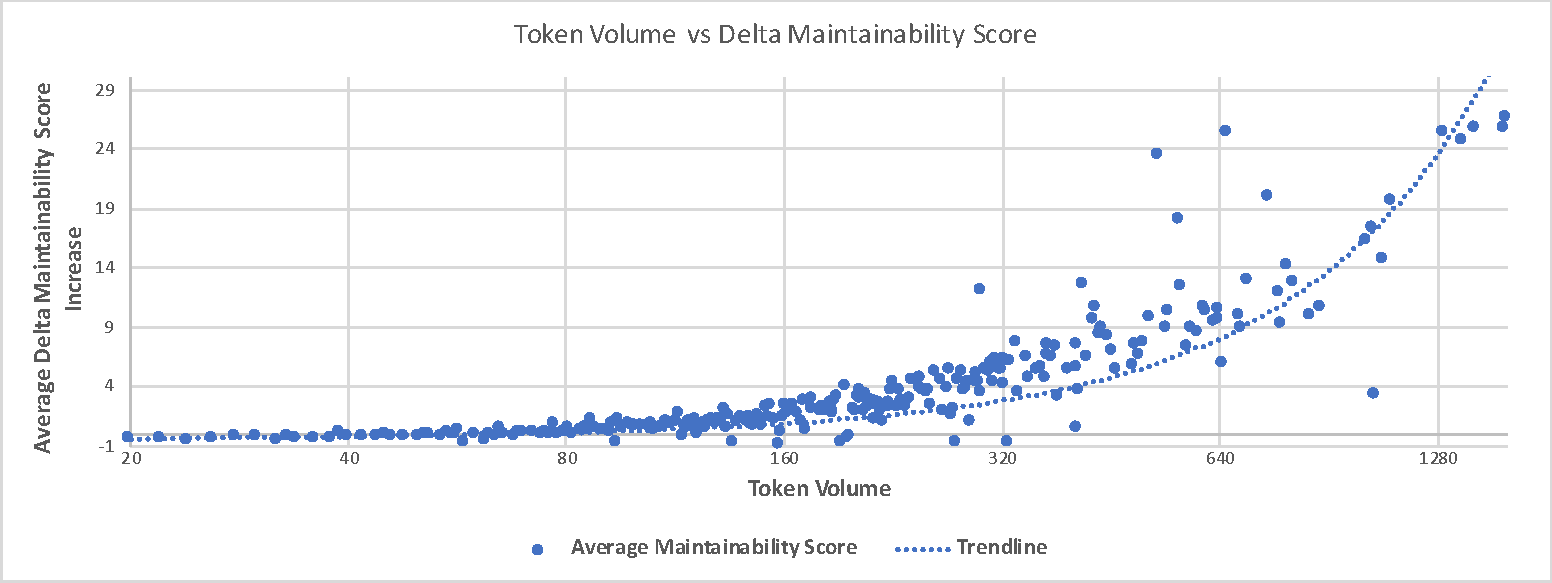
\includegraphics[width=1\textwidth]{img/tokenvolume}
  \caption{A graph that shows how the size in tokens of the refactored clone affects maintainability.}
  \label{fig:maintainabilityscore}
\end{figure*}

\subsubsection{Relation}
Table~\ref{tab:relation_refactor} shows our data regarding how different relations influence maintainability. We have marked rows based on less than 100 refactorings red\todo{not color-agnostic, if printed bw might be a problem --> just make it grey }, as their result does not have statistical significance. Relations are ordered by their scores. \todo{this sentence about relation impact seems more suitable for discussion}Scores do not deviate much (-0.15 to 0.23), indicating that the relation between clones has a minor impact on maintainability. Overall, common hierarchy clones have the highest maintainability, whereas unrelated clones have the lowest maintainability.

\subsubsection{Return Value}
Table~\ref{tab:return} shows how the return value of the extracted method influences the maintainability of the resulting system. The return categories are ordered by their scores. \todo{this sentence about relation impact seems more suitable for discussion}Scores do not deviate much (-0.18 to 0.19), indicating that the return category has a minor impact on maintainability. When the result of the call to the extracted method is directly returned, the maintainability score is the highest. When no value is returned, the maintainability score is the lowest. \todo{this sentence about relation impact seems more suitable for discussion}The main reason that no return value is lowest, is that it is linked to a higher number of parameters required for the extracted method.

\begin{table*}
\centering
\begin{tabular}{@{}lrrrrrr@{}}
\toprule
\textit{\textbf{Return Category}} & \textit{\textbf{Complexity}} & \textit{\textbf{Parameters}} & \textit{\textbf{Size}} & \textit{\textbf{Duplication}} & \textit{\textbf{\#}} & \textit{\textbf{Score}} \\ \midrule
Return & 0.85 & 1.02 & -3.84 & -55.00 & 1,571 & 0.19 \\
Declare & 0.94 & 0.74 & 11.11 & -49.19 & 5,177 & 0.15 \\
\rowcolor[HTML]{FFCCC9}
Assign & 0.79 & 1.07 & 0.43 & -56.29 & 14 & 0.12 \\
Void & 0.76 & 1.49 & -5.85 & -56.35 & 5,921 & -0.18 \\ \midrule
\textbf{Grand Total} & \textbf{0.84} & \textbf{1.12} & \textbf{1.33} & \textbf{-53.26} & \textbf{12,683} & \textbf{0.00} \\ \bottomrule
\end{tabular}
\caption{Average metric values for refactorings of clone classes with the specified return category}
\label{tab:return}
\end{table*}



\subsubsection{Parameters}
Fig.~\ref{fig:arguments} shows how an increase in parameters lowers the maintainability of the refactored code. On the primary x-axis, the maintainability is displayed. The secondary x-axis shows the number of refactorings. The y-axis shows the number of parameters.

\todo{Redo plot, explain axes units}
\begin{figure}[H]
  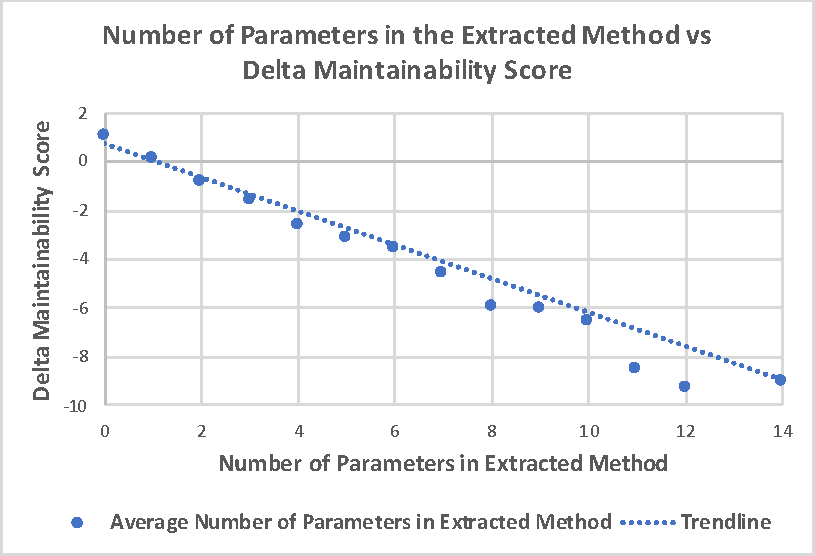
\includegraphics[width=1\columnwidth]{img/arguments}
  \caption{Influence of number of method parameters on system maintainability.}
  \label{fig:arguments}
\end{figure}

\section{Discussion} \label{sec:discussion}
%In this section, we discuss the results of our experiments.

% TODO: Explain about the coupling metric. Discussion: it is not too relevant to the results because most refactorings are SAME CLASS which do not impact on the coupling metric. (maybe more about architectural refactorings because COUPLING, BALANCE, COHESION?)

\subsection{Clone Context}
Regarding clone context, our results indicate that most clones (37\%) are in a common class. This is favorable for \todo{automated?} refactoring because the extracted method does not have to be moved after extraction. 24\% of clones are in a common hierarchy. These refactorings are also often favorable. Another 24\% of clones are unrelated, which is often unfavorable because it often requires a more comprehensive refactoring. 15\% of clones are in an interface \todo{which ...}.

Regarding clone locations, 74\% of clones span part of a method body (77\% if we include constructors). 8\% of clones span several methods, which often require refactorings on a more architectural level. 6\% of clones span only global variables, requiring an abstraction to encapsulate these data declarations. Only 4\% of clones span a full declaration (method, class, constructor, etc.).

\subsection{Extract Method}
28\% of clones can be refactored using the ``Extract Method'' refactoring technique (50\% if we limit our searching scope to method bodies). About 25\% of clones do not span part of a method, therefore they cannot be refactored. Many clones (23\%) do not have a statement as top-level AST-Node. Upon manual inspection, we noticed that the main reason is clones in lambda functions or in anonymous classes. About 15\% of clones span only part of an AST-Node \todo{and?}.

\subsection{Refactoring}
Fig.~\ref{fig:maintainabilityscore} shows an increase in maintainability for refactoring larger clone classes. The tipping point, between a better and a worse maintainable refactoring, seems to lie around a token volume of 63 tokens. There are fewer large clones than small clones, resulting in a very limited \todo{how limited? give the p-value} statistical significance on our corpus when considering clones larger than 100 tokens.

Table~\ref{tab:relation_refactor} shows the results regarding refactorings that are applied to clones with diverse relations. More than 54\% of the refactored clones are in a common class. This is significantly more than the percentage of clones in the common class relation reported in Table~\ref{tab:relation}. The number of refactored unrelated clones is smaller than the number reported in Table~\ref{tab:relation} (24\% -> 18\%). The main reason for this is that refactoring unrelated clones can change the relation of other clones in the same system. If we create a superclass abstraction to refactor an unrelated clone, other clones in those classes that were previously unrelated might become related.

The maintainability scores in Table~\ref{tab:relation_refactor} show that the most favorable clones to refactor are clones with a Sibling relation. The most unfavorable is refactoring clones to interfaces. However, the differences in maintainability in this table are generally small \todo{and?}; according to our data relations have only a minor impact on the maintainability of clones.

Regarding the return type of refactored clones, Table~\ref{tab:return} shows that this has no major impact on maintainability. A method call to the extracted method that is directly returned and no return type extracted methods are slightly more favorable than the others. We think the main reason that the ``Return'' category is on top is that when a variable is declared at the end of the cloned fragment, CR directly returns its value and removes the declaration. This decreases the volume slightly.

% A higher number of parameters directly influences the corresponding metric. 
Fig.~\ref{fig:arguments} shows that more parameters negatively influence maintainability. Not only the \todo{wasn't this a characteristic? this paragraph is somewhat confusing} number of parameters metric is negatively influenced, but more method parameters also increase volume for the extracted method and each of the calls to it. Because of that, we see that the trend of the graph in Fig.~\ref{fig:arguments} decreases relatively rapidly.

\todo[inline]{one paragraph with a general remark on this discussion, summarizing our findings}
\section{Conclusion} \label{sec:conclusion}
\todo[inline]{one paragraph summarizing the context of our research}
We defined automatically refactorable clones and created a tool to detect and refactor them. We measured statistical data with this tool over a large corpus of open-source Java software systems to get more information about the context of clones and how refactoring them influences system maintainability.

We defined two aspects as part of the context of a clone: relation and location. Regarding relations, over 37\% of clones are found in the same class. About 24\% of clones are in the same inheritance hierarchy. Another 24\% of clones are unrelated. The final 15\% of clones have the same interface. Regarding location, over 74\% of clones span part of a method. About 8\% span several methods. Only 4\% of clones span a declaration (method, class, etc.) fully.

We built a tool that can automatically apply refactorings to 28\% of the clones in our corpus using the ``Extract Method'' refactoring technique. 
% The main reason our tool could not refactor all clones is that many clones span certain statements that obstruct method extraction, e.g., when code outside a method is part of a clone.

We measured the change in four maintainability metrics
%before- and after applying each refactoring 
to determine the impact of each refactoring on system maintainability. We found that the most prominent factor influencing maintainability is the size of the clone. We found that the threshold lies at a clone volume of 29 \todo{wasn't this 63?} tokens per clone instance for system maintainability to increase after refactoring the clone. Another factor with a major impact on maintainability is the number of parameters that the extracted method requires to get all required data. We noticed that the inheritance relation of the clone and the return value of the extracted method has only a minor impact on system maintainability.

\bibliographystyle{plain}
\bibliography{references}

\end{document}
